%\subsection{Bloom filter lower bounds}

%\begin{table}[thp]
\begin{center}
  \begin{tabular}{ | c | c |c | c | c | }
    \hline
    Salt & Key & \parbox{.75in}{Private\\ Representation} & \parbox{.75in}{Irreversible\\ Updates} & Result \\ \hline\hline
    0 & 0 & 0 & 0 & Attack 1 \\ \hline
    0 & 0 & 0 & 1 & Attack 1 \\ \hline
    0 & 0 & 1 & 0 & Attack 1 \\ \hline
    0 & 0 & 1 & 1 & Attack 1 \\ \hline
    0 & 1 & 0 & 0 & Attack 2 \\ \hline
    0 & 1 & 0 & 1 & Attack 2 \\ \hline
    0 & 1 & 1 & 0 & Attack 2 \\ \hline
    0 & 1 & 1 & 1 & Attack 2 \\ \hline
    1 & 0 & 0 & 0 & Attack 3 \\ \hline
    1 & 0 & 0 & 1 & Attack 3 \\ \hline
    1 & 0 & 1 & 0 & ? \\ \hline
    1 & 0 & 1 & 1 & Theorem~\ref{thm:bf-priv-salt-bound} \\ \hline
    1 & 1 & 0 & 0 & Attack 4 \\ \hline
    1 & 1 & 0 & 1 & Theorem~\ref{thm:bf-key-bound} \\ \hline
    1 & 1 & 1 & 0 & ? \\ \hline
    1 & 1 & 1 & 1 & Theorem~\ref{thm:bf-key-bound} \\
    \hline
  \end{tabular}
\end{center}
\tsnote{This table feels unintutive, somehow. ``Salt'', ``Key'', ``Irreversible updates'' are all syntactic properties; ``Private Representation'' is an artifact of the attack model.  We need a better way to organize and present these results.}
\caption{Summary table for Bloom filters. \textbf{Attack 1:}The adversary chooses a maximally large test set $\col$ and simulates $\Rep$ to produce a representation $\pub$. The adversary then simulates $\Rep$ for many arbitrarily chosen singleton sets disjoint from $\col$, checking each one to see if its element is a false positive for $\pub$. Once it has accumulated $r$ false positives, call $\REPO$ on $\col$, call $\QRYO$ for each false positive found, and return 1.  \textbf{Attack 2:} The adversary chooses a maximally large test set $\col$ and calls $\REPO$ to produce a representation $\pub$. The adversary then calls $\REPO$ for many arbitrarily chosen singleton sets disjoint from $\col$, using $\QRYO$ on each to determine if its element is a false positive for the representation constructed for $\col$. Once it has accumualated $r$ false positives, return 1. \textbf{Attack 3:}  The adversary chooses a maximally large test set $\col$ and calls $\REPO$ to receive a representation $\pub$ together with the salt $\salt$. Using the known salt, the adversary simulates $\Rep$ for many arbitrarily chosen singleton sets disjoint from $\col$, checking each one to see if its element is a false positive for $\pub$. Once it has accumulated $r$ false positives, call $\QRYO$ for each such false positive and return 1. \textbf{Attack 4:}The adversary chooses a test set $\col_0$ and a target set $\col_1$, performing a search on representable subsets of $\col_0$ represented as a tree ordered by $\subseteq$. Moving up or down in the tree is accomplished using $\UPO$, and at each node $\QRYO$ is called for each element of $\col_1$ to determine which are false positives. Once $r$ false positives are found, halt and return 1. }
\label{tab:main}
\end{table}
\todo{DC (lead)}{Explain away all cases except the one(s) for which we give
security (upperbound) theorems.}
%
The standard Bloom filter shows a variety of different behaviors depending on
its exact implementation. If the hash functions used are chosen beforehand and
potentially known to the adversary, this public information allows offline
attacks to be mounted against the data structure which can produce potentially
damaging false positives. In the case of immutable Bloom filters, making use of
a per-representation salt is sufficient to prevent these attacks, though
depending on the use case the use of non-fixed per-representation randomness may
or may not be feasible. Furthermore, in the case of mutable Bloom filters there
are additional difficulties with offline attacks due to adversarially-chosen
updates. To guarantee correctness in this case we must additionally guarantee
that representations can be kept private from the adversary.

\medskip
\heading{Bit-string operations.}
%
\cpnote{This should be moved to prelims.}
%
For all $m\geq0$ define~$\bmap_m$ as the following function.
For all $\v.x\in[m]^*$ let $\bmap_m(\v.x) = X$, where
$|X|=m$ and $X_v=1$ if and only if $\v.x_i = v$ for some $i\in[|\v.x|]$
%
We call $\bmap_m(\v.x)$ the \emph{bitmap} of~$\v.x$.
%
Let~$X$ and~$Y$ be equal-length bitstrings. We write $X \OR Y$ for their
bitwise-OR, $X \AND Y$ for their bitwise-AND, and $X \XOR Y$ for their
bitwise-XOR. Let $\NOT X = 1^{|X|} \xor X$.
%
Finally, let $\hw(X)$ denote the Hamming wieght of (i.e., the number of 1s in)~$X$.

\subsection{Insecurity of unsalted BFs}
Let $H:\bits^*\to[m]^k$ be a function and consider the following unkeyed
structure constructed from~$H$. Its data objects, supported queries, and
supported updates are as defined in top row of
Figure~\ref{fig:structures-summary}.
%
On input of $\setS\subseteq\bits^*$, the representation algorithm computes
%
\[
  \Rep^H(\setS) = \bigor_{x\in\setS} \bmap_m(H(x)) \,.
\]
%
On input $x\in\bits^*$, the query-evaluation algorithm computes $\Qry^H(M,x) =
[\hw(M \AND \bmap_m(H(x))) = k]$.
%
Lastly, on input of $(M, x) \in \bits^m\by\bits^*$, the update algorithm computes
%
\[
  \Up^H(M,x)= M \OR \bmap_m(H(x)) \,.
\]
%
Let $\BF[H] = (\Rep^H, \Qry^H, \Up^H)$.

\cpnote{WIP}


\ignore{
A generic attack against unsalted, unkeyed data structures handling set
membership queries is for the adversary to choose a large set $\col$ of
potential filter elements and simulate $\REPO$ to produce representations for
$\{x\}$ for each $x \in \col$. Given these, it can perform offline computations
to determine disjoint $\setT$, $\setR \subseteq \col$ such that the elements of
$\setR$ all produce errors when queried for membership in $\REPO(\setT)$. After
a sufficiently large $\setR$ has been found, the adversary makes a single
$\REPO$ call on $\setT$ and makes one $\QRYO$ call per element of $\setR$,
resulting in guaranteed success for the adversary with only a minimal number of
queries performed.

In general, such an attack may not be computationally feasible in the real
world. However, because the attack is entirely offline, many structures with
non-negligible error probabilities are vulnerable to these attacks. For example,
consider a Bloom filter with false positive probability $10^{-5}$ with an
adversary wishing to construct $r = 10$ false positives. The adversary can fix
$\setT$ in advance and perform somewhere on the order of a million hash queries
to random elements in order to construct a $\setR$ of size 10, and then perform
only a single $\REPO$ calls and ten $\QRYO$ calls to the service hosting the
Bloom filter. This is likely to be much more feasible for the adversary than
performing on the order of a million $\QRYO$ calls in an online attack which
randomly guesses elements until it accumulates 10 false positives.
K}

\subsection{Salted BFs in the (im)mutable setting}

The use of a salt without a private key in the public representation setting is
insufficient to defeat this attack. In this setting, the adversary need only
make its $\REPO$ query for $\setT$ in advance, at which point it will receive
both the representation $\pub$ and the salt $\salt$ used to construct it. Using
this known salt, the adversary is still able to simulate $\REPO$ for arbitrary
singleton representations. The previous attack therefore still works with the
same (minimal) number of $\QRYO$ calls at the very end of the experiment, after
it has determined $\setR$ using offline computations.

The opposite of this, using a private key without a salt, does weaken the attack
somewhat. Even with public representations, the adversary cannot locally
simulate $\REPO$ without guessing the private key. However, they can still
outperform random $\QRYO$ calls by making $\REPO$ queries for singleton elements
without fixing any $\setT$ in advance. After selecting a random set $\col$ of
size $q_R-1$, the adversary performs offline computations to find $\setT$,
$\setR \subseteq \col$ such that the elements of $\setR$ are false positives for
the representation of $\setT$ (which can be computed from the representations of
the singleton subsets of $\setT$). The adversary wins if there is a partition
where $\setR$ produces at least $r$ errors on $\REPO(\setT)$.

% ...

Using a salted Bloom filter in the private representation setting, however, does
provide some security. At the time a representation is created, the structure
chooses a salt $\salt$ which it will use for all further queries and updates. In
order for maximum security to be guaranteed, we must ensure that the
representation, and in particular the salt, is kept secret from the adversary.
We define this structure $\SBF[H,k,m,n,\lambda]$ as the Bloom filter structure
that uses $H(s) = (h_1(s),\ldots,h_k(s))$ for hashing inputs to $k$ values in
$[m]$. Furthermore, each call of $\Rep$ first involves picking a salt $\salt$
from the salt space $\bits^\lambda$, and all hashes made to insert or query for
an element $x$ are determined using $H(x \Vert \salt)$. Finally, the parameter
$n$ means that any attempts to represent sets with more than $n$ elements fail.
\todo{DC lead}{Specify what exactly is being analyzed.  What are the updates?}

\begin{theorem}[Correctness Bound for Private-Representation Salted Bloom Filters]\label{thm:bf-priv-salt-bound}
Fix integers $k, m, n, \lambda, r\geq 0$, let $H \colon \bits^* \to [m]$ be a function, and let $\struct_s = \SBF[H,k,m,n,\lambda]$.
  For every $t, q_R, q_T, q_U, q_H \geq 0$, it holds that
  \begin{eqnarray*}
    \Adv{\erreps}_{\struct_\saltybloom,r}(t,&q_R,& q_T, q_U, q_H) \leq \\ && q_R \cdot
     \left[
      \frac{q_H}{2^\lambda} +
      {\dbinom{q_T+q_U}{r}} p(k, m, n+s)^r
    \right] \,,
\end{eqnarray*}
where $s$ is defined to be $\min(r,q_U)$, $H$ is modeled as a random oracle, and $p(k, m, n+s)$ is the standard, non-adaptive false-positive probability on a Bloom filter with the given parameters.
\end{theorem}

This proof first reduces to the single-representation case, which as shown in
lemma~\ref{lemma:errep} will reduce the adversary's advantage by at most a
factor of $q_R$. The main idea behind the proof is to remove the adversary's
adaptivity a step at a time. We isolate the possibility of the adversary
guessing the salt, which would allow it to mount its own offline attack on the
filter without relying on the $\QRYO$ oracle. If the adversary does not guess
the salt, the outputs of the $\REPO$, $\QRYO$, and $\UPO$ oracles are
unpredictable to the adversary, producing uniformly randomly distributed bits to
set (for $\REPO$ and $\UPO$) or to check (for $\QRYO$). Under the assumption
that the adversary does not predict the salt, queries made to distinct elements
are independent of each other. The only remaining issue is that the adversary
can potentially gain an advantage by testing whether some object $x$ is a false
positive for the filter, and then updating the filter to include $x$ only if the
test query returned `false'. An analysis shows that this is now (once imperfect
pseudorandom functions and salt collisions have been dealt with) the only way
for the adversary to gain an advantage over making queries to an immutable Bloom
filter. Because this adaptive strategy introduces tricky conditional
possibilities, we cannot compute an exact value for the adversary's advantage.
Instead, we move to an alternate scenario where each $\QRYO$ also produces a
free update and every $\UPO$ first performs a free query. This makes $\QRYO$ and
$\UPO$ calls indistinguishable, so that the adversary is effectively making a
series of independent random queries that each have a chance to increment the
error counter. Because the number of 1s in the filter can only increase, the
probability of a false positive from any one of these queries is bounded above
by the probability of a false positive on the final maximally-sized filter, a
probability which is given by the Kirsch and Mitzenmacher bound.

\begin{lemma}[In the ROM, salted hashing is almost as good as distinct random functions in \errep1]\label{lemma:salttorand}
  Let $\struct = (\Rep, \Qry, \Up)$ be a data structure with key space $\{\emptystr\}$ and salt space $\bits^\lambda$, and let $\struct'$ be the same structure using true random functions in place of salted hash functions. For every $t, q_R, q_T, q_U, q_H, r \geq 0$, it holds that
  \[
    \Adv{\errep1}_{\struct,r}(t, q_R, q_T, q_U, q_H) \leq \frac{q_H}{2^\lambda} + \Adv{\errep1}_{\struct',r}(t, q_R, q_T, q_U, q_H)
  \]
\end{lemma}

\begin{proof}
Let $\game_0$ be the standard $\errep1$ game for the structure $\struct$, and
let $\game_1$ be the same game for $\struct'$. There exists an adversary $\advB$
such that $\Prob{\game_0(\advA) = 1} \le \Prob{\game_1(\advB) = 1} + q_H/2^\lambda$.
This adversary initializes an empty table $R$ and simulates $\advA$. When a
query $w$ is sent to $\HASHO$, $\advB$ returns $R[w]$ if this entry in the table
is defined. Otherwise, if $w = \langle\salt, x\rangle$ for some
$\salt \in \bits^\lambda$ and $x \in \bits^*$, forward $(\salt, x)$ to $\HASHO$,
store the result in $R[w]$, and return this value. Finally, if $R[w]$ is not
defined and $w$ is not of this form, sample $r$ uniformly from the range of the
hash function, store the result in $R[w]$ and return that result. Queries to all
other oracles are simply forwarded to $\advB$'s oracle. Assuming the output of
the hash function is uniformly distributed, this simulation is perfect unless
$\advA$ guesses the salt correctly, which happens with probability
$q_H/2^\lambda$.
\end{proof}

\begin{figure*}
  \boxThmBFSaltCorrect{0.48}
  {
    \underline{$\game_0(\advA)$}\\[2pt]
      $\col \getsr \advA^H$; $\setC \gets \emptyset$; $\err \gets 0$\\
      $\pub \getsr \Rep[H](\col)$\\
      $\bot \getsr \advA^{H,\QRYO,\UPO}$\\
      return $(\err \geq r)$
    \\[6pt]
    \oraclev{$\QRYO(\qry_x)$}\\[2pt]
      if $\qry_x \in \mathcal{C}$ then return $\bot$\\
      $\setC \gets \setC \union \{\qry_x\}$\\
      $a \gets \Qry[H](\pub, \qry_x)$\\
      if $a \neq \qry_x(\col)$ then $\err \gets \err + 1$\\
      return~$a$
    \\[6pt]
    \oraclev{$\UPO(\up_x)$}\\[2pt]
      $\setC \gets \emptyset$\\
      $a \gets \Qry[H](\pub, \qry_x)$\\
      if $\qry_x \in \setC$ and $a \neq \qry_x(\col)$ then\\
      \tab $\err \gets \err-1$\\
      $\col \gets \col \union \{x\}$\\
      $\pub \gets \Up[H](\pub,\up_x)$\\
      return~$\bot$
    \\[4pt]
    \hspace*{-4pt}\rule{1.043\textwidth}{.4pt}
    \\[5pt]
    \oraclev{$\HASHO_1(\salt,x)$} \hfill\diffplus{$\game_2$}\;{$\game_1$}\hspace*{3pt}\\
      $\hh \getsr [m]^2$; $\vv \gets \fff(\hh$)\\
      if $\salt = \salt^*$ then\\
      \tab $\bad_1 \gets 1$; \diffplus{return $\vv$}\\
      if $T[\salt,x]$ is defined then $\vv \gets T[\salt,x]$\\
      $T[\salt,x] \gets \vv$;
      return $\vv$
  }
  {
    \underline{$\game_1(\advB)$}\\[2pt]
      $\salt^* \getsr \bits^\lambda$;
      $\col \getsr \advB^{\HASHO_1}$\\
      $\pub \gets \Repx[\HASHO_2](\col, \salt^*)$\\
      $\setC \gets \emptyset$;
      $\err \gets 0$\\
      $\bot \getsr \advB^{\HASHO_1,\QRYO,\UPO}$\\
      return $(\err \geq r)$
    \\[6pt]
    \oraclev{$\QRYO(\qry_x)$}\\[2pt]
      if $\qry_x \in \mathcal{C}$ then return $\bot$\\
      $\setC \gets \setC \cup \{\qry_x\}$\\
      $a \gets \Qry[\HASHO_2](\pub, \qry_x)$\\
      if $a \neq \qry_x(\col)$ then $\err \gets \err + 1$\\
      return~$a$
    \\[6pt]
    \oraclev{$\UPO(\up_x)$}\\[2pt]
      $\setC \gets \emptyset$\\
      $a \gets \Qry[H](\pub, \qry_x)$\\
      if $a \neq \qry_x(\col)$ and $\qry_x \in \setC$ then\\
      \tab $\err \gets \err-1$\\
      $\col \gets \col \union \{x\}$\\
      $\pub \gets \Up[\HASHO_2](\pub,\up_x)$\\
      return~$\bot$
    \\[6pt]
    \oraclev{$\HASHO_2(\salt,x)$}\\[2pt]
      $\hh \getsr [m]^2$; $\vv \gets \fff(\hh$)\\
      if $T[\salt,x]$ is defined then\\
      \tab $\vv \gets T[\salt,x]$\\
      $T[\salt,x] \gets \vv$;
      return $\vv$
  }
  {
    \underline{$\game_3(\advB)$}\\[2pt]
    \oraclev{$\QRYO(\qry_x)$}\\[2pt]
      $a \gets \Qry[\HASHO_3](\pub, \qry_x)$\\
      if $a \neq \qry_x(\col)$ then $\err \gets \err + 1$\\
      $\col \gets \col \union \{x\}$
      $\pub \gets \Up[\HASHO_2](\pub,\up_x)$\\
      return~$a$
  }
  {
    \oraclev{$\UPO(\up_x)$}\\[2pt]
      $a \gets \Qry[\HASHO_3](\pub, \qry_x)$\\
      if $a \neq \qry_x(\col)$ then $\err \gets \err + 1$\\
      $\col \gets \col \union \{x\}$
      $\pub \gets \Up[\HASHO_2](\pub,\up_x)$\\
      return~$\bot$
    \\[6pt]
    \oraclev{$\HASHO_i(\salt,x)$}\\[2pt]
      $\hh \getsr [m]^2$; $\vv \gets \fff(\hh$)\\
      return $\vv$
  }
  \caption{Games 0--3 for proof of Theorem~\ref{thm:bf-priv-salt-bound}.}
  \label{fig:bf-priv-salt-bound}
\end{figure*}

\begin{proof}

We first reduce from the $\erreps$ case to the $\erreps1$ case, which by
lemma~\ref{lemma:errep} may scale the adversary's advantage only by a factor of
$q_R$. The game~$\game_0$ is exactly equivalent to the $\erreps1$ experiment, so
$\Adv{\errep1}_{\struct_s,r}(\advA) = \Prob{\game_0(\advA) = 1}$. In~$\game_1$
we split the hash oracle into three, giving the adversary access $\HASHO_1$ in
both stages of the game, while $\HASHO_2$ is reserved for oracular use by
$\Repx$, $\QRYO$, and $\UPO$. For any $\advA$ for~$\game_0$, there is $\advB$
for~$\game_1$ which produces the same advantage by simulating $\advA$. This
adversary first creates its own table $R$ with all values initially undefined.
When $\advA$ makes a query $w$ to $H$, $\advB$ returns $R[w]$ if that entry in
the table is defined. Otherwise, if there are $\salt \in \bits^\lambda$, $j \in
[k]$, and $x \in \bits^*$ such that $w = \langle\salt, j, x\rangle$, forward
$(\salt,x)$ to $\HASHO_1$. For each $j \in [k]$, set $R[\langle\salt, j,
x\rangle] = \vv_j$, where $\vv$ is the output of the $\HASHO_1$ oracle. If there
is no such triple $\langle\salt, j, x\rangle$, just sample $r$ from $[m]$
uniformly and set $R[w] = r$. In either case, return $R[w]$ to $\advA$. When
$\advA$ outputs its collection $\col$, $\advB$ outputs $\col$ as well. Any
queries by $\advA$ to $\QRYO$ or $\UPO$ are forwarded to $\advB$'s corresponding
oracle. The simulation is perfect because $\Rep[H](\col)$ and $\Up[H](\col,\up)$
are identically distributed to $\Rep[\HASHO_2](\col)$ and
$\Up[\HASHO_2](\col,\up)$. Because we have a perfect simulation,
$\Adv{\erreps1}_{\struct_s,r}(\advA) = \Prob{\game_1(\advA) = 1}$.

The game~$\game_2$ is the same as~$\game_1$ until $\bad_1$ is set, which occurs
exactly when $\advB$ sends $(\salt^*,x)$ to $\HASHO_1$ for some $x$. In the
first phase, there is again a $q_1/2^\lambda$ chance of the adversary guessing
the salt. In the second phase, the random sampling used by $\HASHO_i$ ensures
that each call the adversary makes to the $\HASHO_i$ oracle is independent of
all previous calls. We therefore have a $q_2/2^\lambda$ chance of the adversary
guessing the salt during this phase, for a total chance of $q_H/2^\lambda$
chance of the adversary guessing the salt at some point during the experiment.
Then $\Adv{\erreps_1}_{\struct_s,r}(\advA) \le \Prob{\game_2(\advB) = 1} +
q_H/2^\lambda$. Having taken this into account, we may now assume the adversary
never guesses the salt.

We want to show that alternating between sequences of queries and sequences of
updates is no better than making one long series of updates and then one long
sequence of queries. There are three types of updates the adversary can make:
updates to add elements that have been queried and found to be false positives;
updates to add elements that have been queried and found not to be false
positives; and updates to add elements that have not been queried yet. We may
assume without loss of generality that the adversary never makes the first type
of update, since doing so is never beneficial (it does not change the
representation at all and decreases the number of errors the adversary has
found).

Note that the choices of $\vv$ constructed by the $\HASHO_i$ oracles are
independent of all previous queries. Because of this, any update of type 3 is
equivalent to any other update of type 3; the probability of any bit being
flipped by one update is the same as the probability of the bit being flipped by
the other update. Similarly, any update of type 2 is equivalent to any other
update of type 2, but is not the same as type 3 since the probability is
conditioned on $\vv$ not being a false positive. We assume the worst case,
namely that all updates are type 2 (i.e. at least one bit is flipped by each
update).

Because the adversary never guesses the salt, $\HASHO_1$ simply functions as a
random oracle. Furthermore, we can assume the adversary never adds an element of
$\col$ to $\col$ and never makes a $\QRYO$ call for an element which is already
in $\col$, since neither of these provides any additional information and
neither affects the rest of the experiment in any way.

Now we move to the game~$\game_3$. Here each $\QRYO$ query also calls $\UPO$ to
add that element to $\col$. Additionally, the penalty for adding known false
positives is removed. To avoid penalizing the adversary by prematurely maxing
out the number of elements in $\col$ because of added false positives, we also
increase the maximum size of $\col$ from $n$ to $n+s$, where $s = \min(r,q_U)$.
Because the adversary (without loss of generality) stops after accumulating $r$
errors, only $\min(r,q_U)$ false positives will be added to $\col$ and so a
maximum size of $n+s$ is sufficient to produce no penalty for the adversary.
Furthermore, each $\UPO$ call is preceded by a $\QRYO$ call. Neither of these
changes can produce a worse result for the adversary, so $\Prob{\game_2(\advB) =
1} \le \Prob{\game_3(\advB) = 1}$. Now, however, there is no longer any
distinction between $\QRYO$ and $\UPO$ calls. All calls to either oracle are
independent of each other and produce the same effect, querying and then
updating $\col$. Each of these queries for false positives is at most as
successful as a query to a Bloom filter with $n+r$ elements, so the adversary's
probability of finding a false positive on any query is bounded above by the
standard success rate for a Bloom filter with those parameters. The adversary is
required to produce $r$ errors over the course of $q_T+q_U$ queries, which by
the binomial theorem gives an advantage bound of $\Prob{\game_3(\advB) = 1} \le
\binom{q_T+q_U}{r}p(k, m, n+s)^r$.

The full adversarial advantage is then
$$\Adv{\erreps_1}_{\struct_s,r}(\advA) \le q_R \cdot \left(\frac{q_H}{2^\lambda} + \binom{q_T+q_U}{r}p(k, m, n+s)^r\right).$$

%\missingqed
\end{proof}

If we use both a salt and a key together with a built-in threshold, we can attain a good error bound even in the public-representation case. In particular, this proof eliminates the need for a factor of $q_R$.

\begin{theorem}[Correctness Bound for Salted and Keyed Bloom Filters]\label{thm:bf-key-bound}
Fix integers $k, m, \lambda, r\geq 0$ and a threshold $p \in [0,1]$, let $\Pi$ be the salted and keyed Bloom filter described above with PRF $F$, and let $d$ be the error function assigning a weight of 1 to a false positive and 0 to a correct response.
  For every $t, q_R, q_T, q_U, q_H \geq 0$ such that $q_T \geq r$, it holds that
  \begin{eqnarray*}
    \Adv{\errep}_{\struct,r,d}(t,&q_R,& q_T, q_U, q_H) \leq \\ && \Adv{\prf}(F) + q_R^2/2^\lambda + I_{(n/m)^k}(r, q_T-r+1) \,.
  \end{eqnarray*}
where $I$ is the regularized incomplete beta function.
\end{theorem}

\begin{figure*}
  \boxThmBFSaltCorrect{0.48}
  {
    \underline{$\game_0(\advA)$}\\[2pt]
      $\key \getsr \keys$; $i \gets 0$\\
      $\bot \getsr \advA^{\HASHO,\REPO,\QRYO,\UPO}$\\
      return $[\sum \err \geq r]$
    \\[6pt]
    \oraclev{$\REPO(\col)$}\\[2pt]
      $i \gets i + 1$\\
      $\col_i \gets \col$\\
      $\pub_i \gets \Rep_K[\HASHO](\col)$\\
      return $\pub_i$
    \\[6pt]
    \oraclev{$\QRYO(i,\qry_x)$}\\[2pt]
      $a \gets \Qry[\HASHO](\pub_i, \qry_x)$\\
      if $a \neq \qry_x(\col)$ then $\err_i[x] \gets 1$\\
      return~$a$
    \\[6pt]
    \oraclev{$\UPO(i,\up_x)$}\\[2pt]
      $a \gets \Qry[\HASHO](\pub_i, \qry_x)$\\
      if $\err_i[x] = 1$ then $\err_i \gets 0$\\
      $\col_i \gets \col_i \union \{x\}$\\
      $\pub_i \gets \Up[\HASHO](\pub_i,\up_x)$\\
      return~$\pub_i$
    \\[4pt]
    \oraclev{$\HASHO(x)$}\\[2pt]
      return $H(x)$
    %\hspace*{-4pt}\rule{1.043\textwidth}{.4pt}
  }
  {
  \underline{$\game_1(\advB)$}\\[2pt]\\
    \oraclev{$\HASHO(i,x)$}\\
      if $T[i, x]$ is $\undefn$ then $T[i, x] \getsr [m]^k$\\
      return $T[i, x]$
    \\[6pt]
    \underline{$\game_2(\advB)$}\\[2pt]\\
      $\key \getsr \keys$; $i \gets 0$; $\setC \gets \emptyset$\\
      $\bot \getsr \advA^{\HASHO,\REPO,\QRYO,\UPO}$\\
      return $[\sum \err \geq r]$
    \\[6pt]
    \oraclev{$\QRYO(\qry_x)$}\\[2pt]
      do\\
      $\tab y \getsr \mathcal{X}$\\
      while $y \in \col \cup \setC$\\
      $a \gets \Qry[\HASHO](\pub_i, \qry_y)$\\
      if $a \neq \qry_y(\col)$ then $\err_i[y] \gets 1$\\
      return~$a$
  }
  {
  }
  {
  }
  \caption{Games 0--2 for proof of Theorem~\ref{thm:bf-priv-key-bound}.}
  \label{fig:bf-priv-salt-bound}
\end{figure*}

\begin{proof}

The key to the proof is that seeing the representation of a salted, keyed Bloom
filter does nothing to tell the adversary about what the responses to $\QRYO$
will be. Using a conditioning argument, we move from $\game_0$, which is
equivalent to the standard $\errep$ game, to the alternate $\game_1$ that uses a
lazily-evaluated random function in place of the PRF $F$ for hashing, with the
random function being different for each representation. Provided that the
adversary cannot distinguish the PRF from a random function and provided that
the per-representation salt never repeats (the probability of which is on the
order of $q_R^2/2^\lambda$ by the birthday bound), the adversary cannot
distinguish this from the original game. By a conditioning argument, then, we
have $\Adv{\game_0}_{\struct,r}(\advA) \le \Adv{\prf}(F) + q_R^2/2^\lambda + \Adv{\game_1}_{\struct,r}(\advA)$.

Next, since it never benefits the adversary to re-query an element instead of
querying a new one, and because false negatives do not occur in Bloom filters,
we can assume without loss of generality that the adversary only makes queries
to previously-unqueried elements which are not in the underlying set. But if an
element is not in the underlying set, it must not have been included in the
original $\col$ sent to $\REPO$, and it must never have been inserted with
$\UPO$ since Bloom filters do not support deletion. Furthermore, since it has
not been queried before, it has not been tested with $\QRYO$ either. This means
that each element being queried is a new input to the random function used for
hashing, and its output is therefore indistinguishable from any other input that
is provided. We can then move from $\game_1$ to $\game_2$, which ignores the
query given as input and instead makes a random query to a previously-untested
element. Since the outputs of the $\QRYO$ oracle are indistinguishable from
those in $\game_1$ and there are no other changes, we have
$\Adv{\game_1}_{\struct,r}(\advA) = \Adv{\game_2}_{\struct,r}(\advA)$. But now
that the queries are random, the adversary cannot possibly do better than
producing a representation with maximal (non-adaptive) false-positive
probability and making as many arbitrary queries as possible. Given a threshold
where the proportion of 1 bits is capped at $p$, the false positive probability
for each query is bounded by $p^k$. By the properties of the binomial
distribution, the probability of accumulating at least $r$ errors given $q_T$
queries is
$$\Adv{\errep}_{\struct,r,d}(\advA) \le \Adv{\prf}(F) + q_R^2/2^\lambda + I_{p^k}(r, q_T-r+1)$$

\end{proof}

%We can use this final and best bound to demonstrate some of the possible bounds
%with various parameter settings. Figure ? shows the upper bound for a various
%combination of parameters, starting from the default parameters of $k = 4$, $m =
%1024$, $n = 100$, $r = 10$, $q_R = 1$, $q_T = 100$, and $q_U = 100$. The most
%significant factor in the adversarial advantage is $q_R$, with even small
%increases producing a drastic increase in the adversarial advantage. Since this
%is the only part of the error bound that is not clearly associated with an
%attack, it is possible that this term could be reduced or eliminated.

%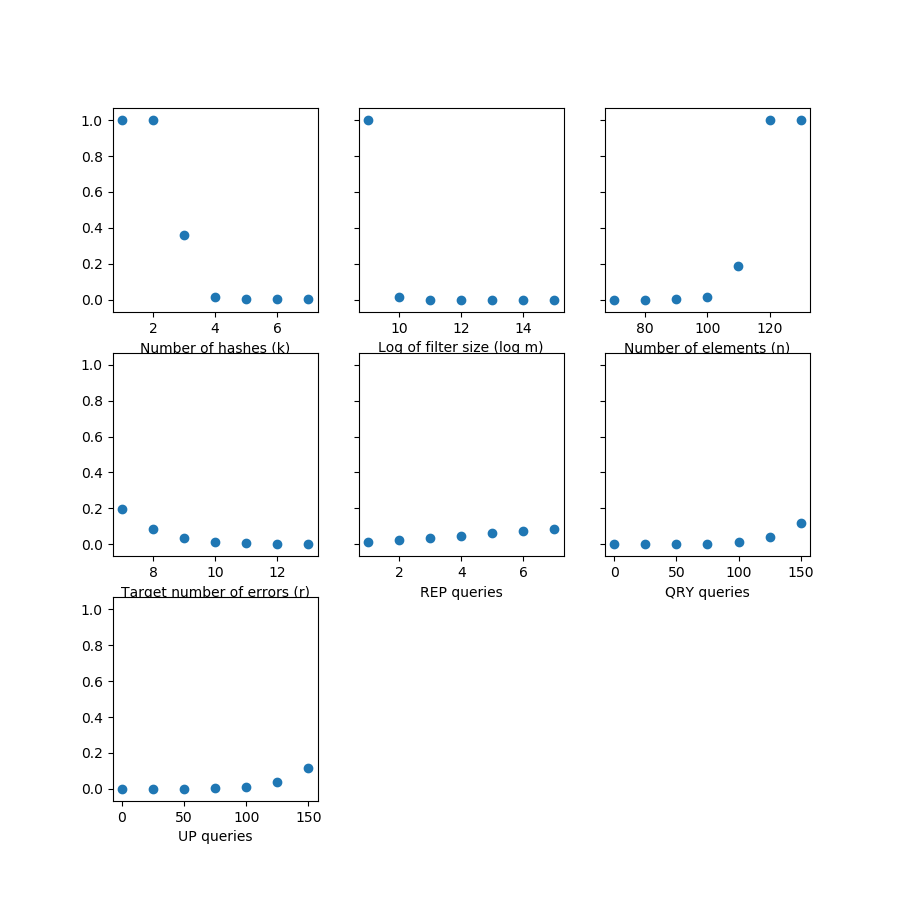
\includegraphics[scale=0.75]{BF_Fig}